% Prose for Section 5 onwards. Numbers come from results_macros.tex, which is
% regenerated from outputs/all_results.json by report/make_tables.py, so this
% text stays in sync with the actual runs.

All five configurations ran the full 25 epochs. The baseline C1 reaches
\CfgOneBit\% bit accuracy and reconstructs \CfgOneSeq\% of 32-character segments
exactly. Among C1 to C4 the ablation separates good models from slightly better
ones, so those differences are small but move consistently across every metric.
C1 fails in short local bursts on rare words, turning \texttt{Dynasty} into
\texttt{Dylesty}: one mispredicted BPE token rewrites several characters at once,
and since pieces are variable-length it also shifts everything after it. This is
why sequence accuracy is far harsher than bit accuracy throughout, as one bad
token forfeits the whole segment.

\begin{figure}[t]
\centering
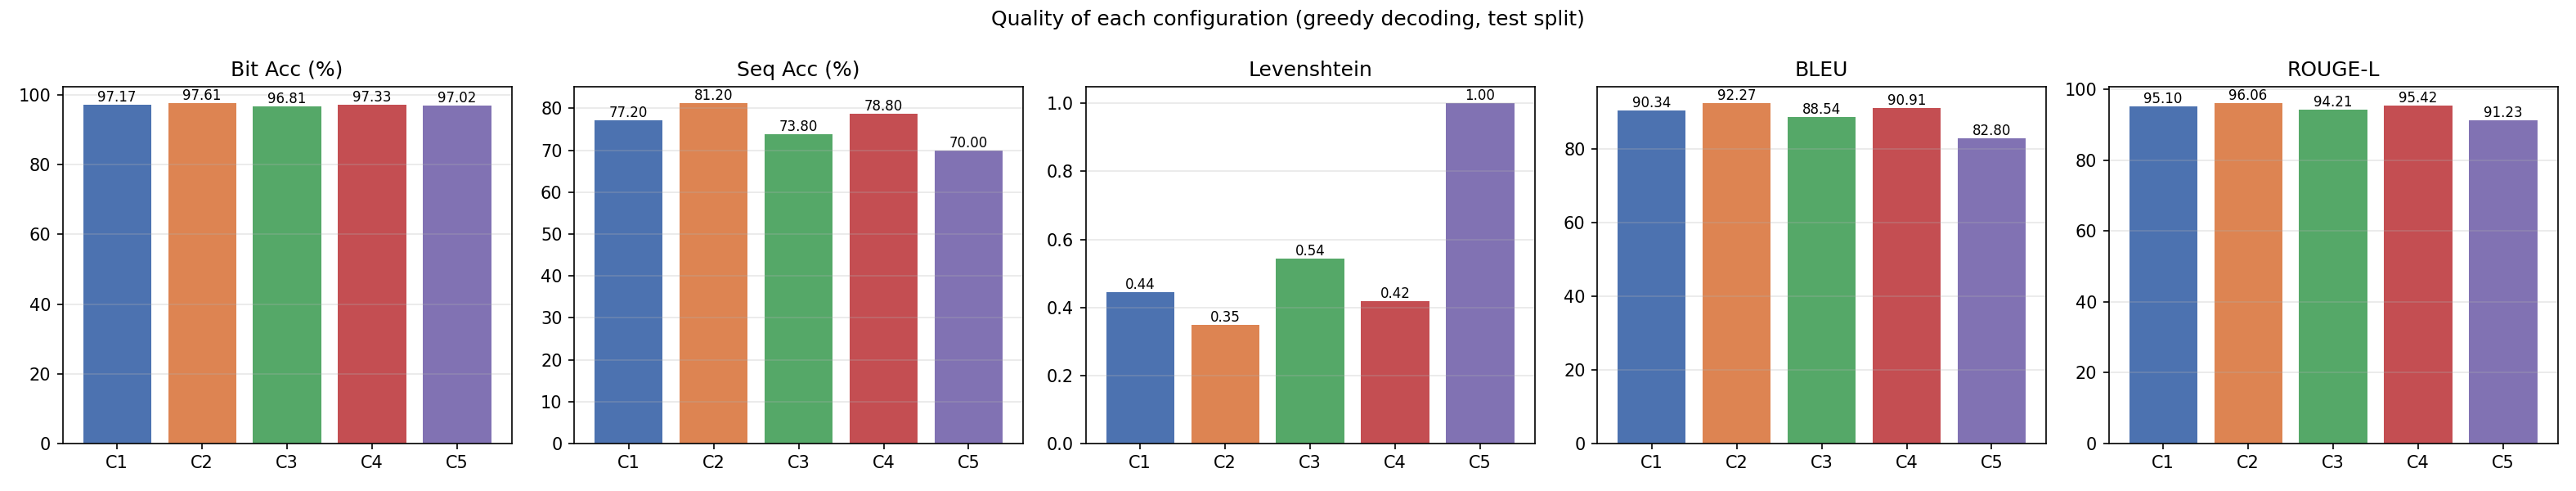
\includegraphics[width=\linewidth]{ablation_quality.png}
\caption{Decoding quality across the five configurations.}
\label{fig:quality}
\end{figure}

\subsection{C2: RoPE improves every quality metric for free}

Rotary embeddings give the largest gain among the tokenised models. Sequence
accuracy rises from \CfgOneSeq\% to \CfgTwoSeq\%, a \textbf{4.0-point absolute
improvement}, with bit accuracy \CfgTwoBit\%, edit distance \CfgTwoLev, and BLEU
up from \CfgOneBleu\ to \CfgTwoBleu. This costs \textbf{zero parameters}
(\CfgTwoPar\,M, identical to C1) and \textbf{zero extra memory} (\CfgTwoMem\,MB
against \CfgOneMem\,MB): RoPE adds no learnable weights, only a deterministic
rotation of $q$ and $k$.

This fits the task. By Eq.~\ref{eq:cipher} the output at position $i$ depends on
$i \bmod 8$, so the decoder needs not \emph{where} it is absolutely but \emph{how
far} it has advanced relative to the source it consumes, which is what RoPE
encodes: the logit is a function of the offset $m-n$ alone. The cost is
throughput, \CfgTwoSec\,s per epoch against \CfgOneSec\ (7.6\% slower); decoding
is unaffected, as the tables are precomputed.

\subsection{C3: GQA trades accuracy for parameters and decode speed}

GQA worsens every quality metric: sequence accuracy \CfgThreeSeq\% ($-3.4$
points), bit accuracy \CfgThreeBit\%, edit distance \CfgThreeLev. Collapsing 8
key/value heads to 2 removes \textbf{0.89\,M parameters} ($-11.6$\%) and forces
four query heads to share one key/value subspace, so the model represents fewer
distinct ways of matching queries against keys. Where the decoder must attend to
a precisely located 8-bit window, that lost specificity is not free. What GQA
buys is inference cost: decoding drops to \CfgThreeGen\,s ($-7.6$\%) and peak
memory to \CfgThreeMem\,MB, as the KV-cache shrinks fourfold.

One detail is easy to misread: C3 is \emph{slower} to train than C1
(\CfgThreeSec\ against \CfgOneSec\,s per epoch) despite having fewer parameters.
Under teacher forcing there is no KV-cache to shrink, so only the broadcast of 2
key/value heads back to 8 remains, which is pure overhead. GQA is an
\emph{inference-time} optimisation, and this experiment separates the two regimes.

\subsection{C4: RMSNorm is a strict improvement}

RMSNorm improves quality \emph{and} reduces cost on every axis at once. Sequence
accuracy rises to \CfgFourSeq\% ($+1.6$ over C1) and bit accuracy to
\CfgFourBit\%, while epoch time falls to \CfgFourSec\,s (7.7\% faster, quickest
of all five), peak memory to \CfgFourMem\,MB ($-6.0$\%), and decoding to
\CfgFourGen\,s ($-14.9$\%). Dropping mean-subtraction removes a full reduction
over the feature axis in both passes, and dropping the bias explains the small
parameter difference. The accuracy gap is within run-to-run noise (perplexities
\CfgFourPpl\ and \CfgOnePpl), so the honest reading is not ``RMSNorm is more
accurate'' but ``\textbf{re-centring contributes nothing measurable here, and its
cost is real}.'' Pre-norm streams are already approximately zero-mean.

% =====================================================================
\section{The token-free trade-off (C5)}
\label{sec:blt}

C5 is the only configuration that changes the input representation rather than a
computation inside the network, and the only one that loses to the baseline.
Sequence accuracy falls to \CfgFiveSeq\% against C1's \CfgOneSeq\%, a
\textbf{7.2-point drop}, edit distance more than doubles to \CfgFiveLev, and BLEU
falls to \CfgFiveBleu, yet bit accuracy is essentially unchanged
(\CfgFiveBit\%). The model gets the bytes right and assembles them badly.

\paragraph{Right bytes, wrong places.} C5 has the \emph{lowest} teacher-forced
perplexity of all five (\CfgFivePpl\ against \CfgOnePpl) yet the worst sequence
accuracy: given the correct prefix the next byte is almost determined, but under
free-running decoding it is weakest, so the errors are about \emph{where} a byte
belongs rather than \emph{which} one. C5 turns \texttt{half of the Mi} into
\texttt{off hald the M}, the right characters reordered with an insertion pushing
the rest out of phase, and one such slip forfeits the segment.

\paragraph{Why entropy patching is a poor fit \emph{here}.} By
Eq.~\ref{eq:cipher} the task is byte-local and rigidly aligned: after packing,
output byte $i$ depends on source byte $i$ and on $i \bmod 8$, so the ideal model
learns a fixed diagonal correspondence. Entropy patching is instead
\emph{content}-driven, and the two sides are cut at unrelated places: cipher
bytes are near-uniform ($H_0 = 6.04$ bits, threshold 4.94) so their boundaries
are near-arbitrary, while plaintext is English ($H_0 = 4.34$, threshold 3.98) and
breaks at word-like positions. Neither respects the key period of 8 nor aligns
with the other, so the bottleneck must rebuild a strict one-to-one correspondence
across boundaries that do not correspond. This reflects the interaction between
mechanism and task, not a defect of the mechanism: on natural language the same
procedure is what makes BLT work.

\paragraph{Cost.} Packing the bits makes the stream 32 bytes rather than 256, and
entropy patching compresses that to about 10.3 patches, so C5's global
transformer runs on a \emph{shorter} sequence than C1's 23 BPE tokens. Peak memory
is nevertheless \CfgFiveMem\,MB against \CfgOneMem\,MB ($1.41\times$): the saving
is outweighed by the byte-level periphery, two extra local stacks over the
34-byte stream plus the dense masks variable-length pooling needs. Epoch time is
\CfgFiveSec\,s ($1.93\times$) and decoding \CfgFiveGen\,s ($4.15\times$), as 32
bytes are emitted one at a time instead of roughly 21 tokens. The one clear win is
size: C5 has the \textbf{fewest parameters} (\CfgFivePar\,M), since dropping the
vocabulary deletes two $4096 \times 256$ embedding matrices.

% =====================================================================
\section{Conclusion}

\textbf{RoPE} buys $+4.0$ points of sequence accuracy for no parameters and no
memory; \textbf{GQA} costs 3.4 points and is \emph{slower} to train, its benefit
being a KV-cache effect teacher forcing never exercises; \textbf{RMSNorm} is free
on every axis; and the \textbf{token-free BLT} costs 7.2 points at $1.41\times$
memory and $4.15\times$ decode time, with the fewest parameters. \looseness=-1
The three changes \emph{inside} the network are small and roughly free, while the
change to the \emph{representation} dominates, its sign depending on whether it
respects the mapping's structure. BPE merges cut across the byte boundaries this
cipher is defined on, so C1 makes substitution errors; entropy patches cut the
sides at unrelated positions, so C5 makes positional ones. A representation is
good or bad only relative to the alignment a task demands.
